\chapter{Parametric Loudspeaker Array}
%\clearpage
\section{Introduction}
Parametric loudspeaker arrays are transducer arrays, which use the demodulation of ultrasound in air to generate a highly directional and steerable sound source. This effect was first discovered by Westerveld \cite{doi:10.1121/1.1918525} and used in a loudspeaker, the \mbox{\textit{Audio Spotlight}}, by Masahide Yoneyama and Jun‐ichiroh Fujimoto \cite{doi:10.1121/1.389414}.

Why ultrasound generates a higher directivity is shown in Section \ref{3_sec:directivity}, how the demodulation works in Section \ref{3_sec:demodulation} and how signal processing methods can be applied to improve the audio quality and enable beam steering capabilities are shown in Section \ref{3_Parametric_array_Sec:Modulation} and Section \ref{3_Parametric_array_Sec:Array_signal_processing}.
\section{Directivity of Ultrasonic Transducers}\label{3_sec:directivity}
As mentioned, ultrasonic transducer produce a highly directional beam. In this chapter the mathematical foundations for this effect will be laid. 
The simplest model of a transducer is to think of it as a slit on which an incoming planar sound wave is diffracted on.\cite{alma99116706330905515} 

The far-field air pressure of a transducer, explained in Section \ref{2_subsec:single_slit}, can be calculated in relation to the angle and distance as 
\begin{equation}
    p(\varphi,r) 
    = 
    \frac{A}{r} \underbrace{\frac{\sin \left ( \frac{ka \sin \phi}{2}\right )}{ \frac{ka \sin \phi}{2}}}_{D_T(\varphi)}.
\end{equation}
Where the sinc function is better known as the directivity of the transducer.
\begin{equation}
    D_T(\varphi) = \frac{\sin \left ( \frac{ka \sin \phi}{2}\right )}{ \frac{ka \sin \phi}{2}}.
\end{equation}
This directivity for an acoustic wave radiated by a loudspeaker size of $a = 16 \, \text{mm}$ is shown in Figure \ref{2_subfig:single_slid_amp}. 
It is important to keep in mind that this directivity is just a model and the true directivity of a transducer can vary massively depending on its geometry, especially as the angle increases.

\section{Demodulation Process}\label{3_sec:demodulation}
The most fundamental equation for modeling the non linear behaviour of air is the \acrfull{kzk} equation \cite{MIT_Ultrasound} given as
\begin{equation}
    \frac{\partial^2 p}{\partial z \partial \tau} 
    = 
    \frac{c_0}{2} \nabla^2_rp
    + 
    \frac{\delta}{2c_0^3}\frac{\partial^3 p}{\partial \tau^3} 
    + 
    \frac{\beta}{2\rho_0c_0^3}\frac{\partial^2 p^2}{\partial \tau^2},
\end{equation}
of which analytical solutions cannot be calculated.
However, the solution can be approximated by first solving for the linear ultrasonic field $p_1$ by setting the nonlinear term to zero $\beta = 0$ and then solve for the nonlinear solution $p_2$. The final solution is then the superposition of these two fields $p = p_1 + p_2$.
The ultrasonic field $p_1$ is described by 
\begin{equation}
     \frac{\partial^2 p_1}{\partial z \partial \tau} 
    = 
    \frac{c_0}{2} \nabla^2_rp_1 
    + 
    \frac{\delta}{2c_0^3}\frac{\partial^3 p_1}{\partial \tau^3} 
\end{equation}
and this can now analytically be solved. 
This solution then can be used as an approximation for the non linear part of the equation
\begin{equation}
     \frac{\partial^2 p_2}{\partial z \partial \tau} 
    = 
    \frac{c_0}{2} \nabla^2_rp_2 
    + 
    \frac{\delta}{2c_0^3}\frac{\partial^3 p_2}{\partial \tau^3} 
    + 
    \frac{\beta}{2\rho_0c_0^3}\frac{\partial^2 p_1^2}{\partial \tau^2}
\end{equation}
which can now be solved near the axis analytically.
The resulting function $p_2$ turns out to be 
\begin{equation}
    p_2 = \frac{\beta P_0^2 a^2}{16 \rho_0 \alpha c_0^4 a^2}\frac{d^2}{dt^2} E^2(t).
\end{equation}
Where $E(t)$ is the enveloping of the output signal of the transducers. 
This means that the  pressure of the wave in the far-field is proportional to the second derivative of the squared modulated signal.
\begin{equation}
    p_2 \propto \frac{d^2}{dt^2} E^2(t).
\end{equation}
If the pressure now should be the desired audio signal $f(t)$, the envelope of the output signal of the transducers has to be
\begin{equation}
    E(t) = \sqrt{\left ( 1 + m \int \int f(t)dt^2 \right )} =  \sqrt{\left ( 1 +x^2 \right )}.
\end{equation}
But it transpires that this is impossible to accomplish because of the limited bandwidth of the ultrasonic transducers.
If $E(t)$ is written as a Taylor approximation
\begin{equation}\label{3_eq:ideal_envelope}
    E(t) 
    = 
    \frac{1}{A} \left ( 1 + \frac{1}{2}x - \frac{1}{8}x^2 + \frac{1}{16}x^3 - \dots \right ) 
    =
    1 - \sum_{k=0}^\infty \frac{2}{k+1} \left ( \binom{2k}{k} \right) \left ( -\frac{x}{4}\right )^{k+1}.
\end{equation}
The spectrum $E_T(\omega)$ of the optimal signal is
\begin{equation}
    E_T(\omega) = \frac{1}{A} \left ( 1 + \frac{1}{2}X(w) - \frac{1}{8}\left (X(w) * X(w)\right ) \pm \dots \right ).
\end{equation}
This shows that $E_T(\omega)$ has an infinite bandwidth, because each correlation in frequency, or multiplication in time, doubles the bandwidth.
So an approximation for the envelope has to be found.
\newpage

\section{Modulation Process}\label{3_Parametric_array_Sec:Modulation}
Due to the finite bandwidth of transducers and the infinite bandwidth of the ideal envelope, as shown in Section \ref{3_sec:demodulation}, an approximation for the envelope has to be made.\\
Figure \ref{3_fig:block_diagram_modulation} shows the modulation and demodulation process.

\begin{figure}[h!]
    \centering
    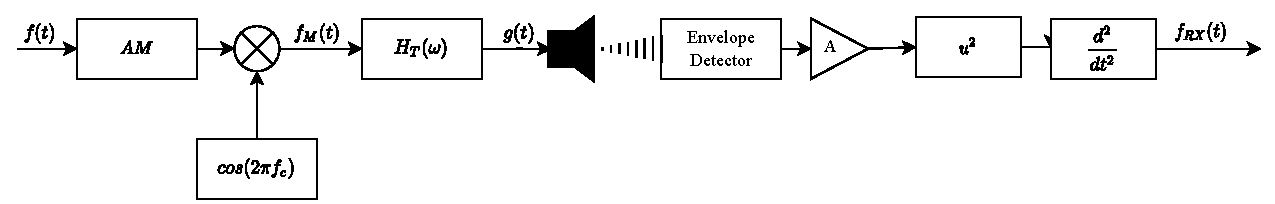
\includegraphics[width=\textwidth]{images/3_Parametric_array/Modulation_Demodulation_Process.pdf}
    \caption{Block Diagram of Modulation and Demodulation Process}
    \label{3_fig:block_diagram_modulation}
\end{figure}

Following, two possible modulation methods are presented.  
\subsection{Amplitude Modulation}
One possible approximation is to use regular amplitude modulation. The emitted signal $g_{AM}(t)$ would be 
\begin{equation}
    g_{AM}(t) = h_T(t) * (1 + mf(t)).
\end{equation}
Often $H_T(\omega)$ is approximated to be $\frac{1}{s^2}$, due to the narrow bandwidth of the \acrshort{put}, which would cancel out the second derivative
\begin{equation}
    f_{RX}(t) 
    = 
    Ag^2_{AM}(t) 
    =
    A(2mf + m^2f^2(t))
    =
   \underbrace{2Amf(t)}_{\text{Signal}} + \underbrace{2Am^2f^2(t)}_{\text{Distortion term}}.
\end{equation}
If the simplification of $H_T(\omega)$ is not made the spectrum of the received signal becomes
\begin{equation}
    F_{RX}(\omega) = 2A(mF(\omega)H(\omega) + m^2(F(\omega)*F(\omega))H(\omega)).
\end{equation}
As can be seen the modulation index $m$ is squared inside of the distortion term and only linear in the signal. This means that if the modulation index would be chosen small enough the distortion term would vanish, but the power of the signal would also be reduced significantly. 
\subsection{Modified Amplitude Modulation}
As seen, if \acrshort{am} is used, there is a problematic distortion term. \acrfull{mam} uses a similar idea to \acrfull{qam} to get rid of this problem \cite{MAM_Main_Paper} .
As inphase component the input signal $1 + mf(t)$ with a \acrshort{dc} offset is used and as the quadrature component the signal $\sqrt{1 - m^2f^2(t)}$ is used. If now the output signal of the modulation $f_M(t)$ is calculated, as described in \ref{2_QAM_sec:QAM}, it turns out to be
\begin{equation}
    f_M(t) = \sqrt{2 + 2mf(t)} \sin{\left(2 \pi f_c t + \arctan{ \left ( \frac{\sqrt{1 - m^2f^2(t)}}{1 + mf(t)} \right )} \right )}.
\end{equation}
If $H_T(\omega)$ is now again assumed to be $H_T(\omega) = \frac{1}{\omega^2}$, the signal turns out to be exactly what is should be. 

This modulation method seems to be optimal, but again because of the square root in the quadrature component it cannot be produced due to the limited bandwidth of ultrasonic transducers. However, the basic idea still can be used. This is done by approximating the distortion terms with a Taylor series
\begin{equation}
    Q(t) 
    = 
    \sqrt{1 - m^2f^2(t)}
    = 
    \sum_{i=0}^\infty \frac{(2i)!}{(1-2i) i!^2 4^i}m^{2i}f^{2i}(t) 
    \approx 
    \sum_{i=0}^k \frac{(2i)!}{(1-2i) i!^2 4^i}m^{2i}f^{2i}(t).
    \label{3_eq:mam_distortion_approx}
\end{equation}
Depending on the frequency response of the transducers the degree of the approximation $k$ can be chosen. The higher the degree of approximation becomes, the higher the bandwidth of the transducers has to be.
\newpage

\section{Array Signal Processing}\label{3_Parametric_array_Sec:Array_signal_processing}
The theory in this section is mostly taken from the book Fundamentals of Ultrasonic Phased Array \cite{alma99116706330905515}.
\subsection{Phased Array Beam Model}\label{3_subsec:phased_array_model}
To explain phenomena such as beam steering and beam focusing the phased array beam model has to be introduced.
 \begin{figure}[h!]
     \centering
     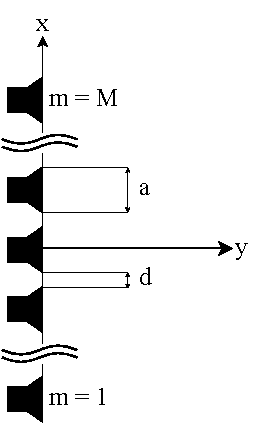
\includegraphics[width=0.3\textwidth]{images/3_Parametric_array/Transducer_Arangement.pdf}
     \caption{Transducer Arrangement}
     \label{3_Parametric_array_img:Transducer_Model}
 \end{figure}
Figure \ref{3_Parametric_array_img:Transducer_Model} shows the basic setup of a transducer array with M elements, where $M$ is odd. The position of the mth element is given as \cite{alma99116706330905515} 
\begin{equation}\label{3.4_eq:simplified_xm}
    x_m 
    = 
    \left ( \frac{2m -1 - M}{2} \right ) \underbrace{(d + a)}_{s}
    =
    \left ( \frac{2m -1 - M}{2} \right ) s,
\end{equation}
where $d$ is the distance between the transducers, $a$ is the size of the transducers and $s$ is known as the pitch of the array. 
The far field pressure of a single element can be calculated as \cite{alma99116706330905515}
\begin{equation}
    p_m(r_m,\omega) 
    =
    \underbrace{\rho c V_0 \frac{k a}{2 M} \sqrt{\frac{2}{\pi i}}}_{A} D_T(\varphi_{m}) \frac{e^{j k \frac{a}{2} r_m}}{\sqrt{k \frac{a}{2} r_m}}, 
\end{equation}
where
\begin{equation}
    r_m
    = 
    \sqrt{\left ( \frac{2x}{a} - \frac{2x_m}{a}\right )^2 + \left ( \frac{2y}{a} \right )^2}
\end{equation}
and 
\begin{equation}
    \varphi_m = \sin^{-1}{\left ( 2\frac{x - x_m}{a r_m} \right )}.
\end{equation}
If now each element gets its own weighting factor $C_m$ and a phase delay $\Delta t_m$ the pressure can be calculated as 
\begin{equation}
    p(r_m,\omega) 
    = 
    A \sum_{m=1}^M C_m e^{j\omega \Delta t_m}  D_T(\varphi_{m}) \frac{e^{j k \frac{a}{2} r_m}}{\sqrt{k \frac{a}{2} r_m}}.
\end{equation}
\subsubsection{Far Field}
If only the far field is of interest. Then $r_{m}$ can be simplified to \cite{alma99116706330905515}
\begin{equation}
    r_{m} = R - x_m \sin{\varphi},
\end{equation}
and $\varphi_m$ to
\begin{equation}
    \varphi_m = \varphi.
\end{equation}
So the pressure can be approximately written as
\begin{align}
    p(R,\varphi,\omega) 
    &= 
     A D_T(\varphi) \underbrace{\frac{e^{j k R}}{\sqrt{k R}}}_{P(R)} \sum_{i=0}^M C_m e^{j\omega \Delta t_m}e^{-jkx_m\sin{(\varphi)}} \\
    &= 
    A D_T(\varphi) P(R) \sum_{i=1}^M C_m e^{j(\omega \Delta t_m - kx_m\sin{(\varphi)})}.
\end{align}
Or with \ref{3.4_eq:simplified_xm} as
\begin{equation}
    p(R,\varphi,\omega) 
    = 
    A D_T(\varphi) P(R) \underbrace{\sum_{i=1}^M C_m e^{j (\omega \Delta t_m -k \left ( \frac{2m -1 - M}{2} \right )s \sin{(\varphi)} )}}_{D_S(\bm{C}, \bm{\Delta t} , \varphi)}.
    \label{3_eq:beam_model_final}
\end{equation}
This is the main model used to explain the directivity pattern of parametric transducer arrays. The sum can be understood as an array directivity $D_s$ introduced by the delays and weights. 

As an example the weights are set to $C_m = 1$ and the delays to $\Delta t_m = 0$. This leads to
\begin{equation}
   D_s(\phi)
    = 
    e^{jks\left ( \frac{M+1}{2} \right )\sin{\phi} } \sum_{m=1}^M \left ( e^{-jks \sin{(\varphi)}} \right ) ^ m .
\end{equation}
This can be seen as a geometric series which can be written as 
\begin{align}
   \sum_{m=1}^M \left ( e^{-jks \sin{(\varphi)}} \right ) ^ m
    &= 
     e^{-jks \sin{(\varphi)}}\frac{1 - e^{-jks \sin{(\varphi) M }}}{1 - e^{-jks \sin{(\varphi)}}} \\
     &=
     e^{-jks\left ( \frac{M + 1}{2}\right ) \sin{(\varphi)}} \frac{\sin{\frac{Mks\sin{(\phi)}}{2}}}{\sin{\frac{ks\sin{(\varphi)}}{2}}}.
\end{align}
The array directivity can be described as
\begin{equation}
    D_s(\phi) 
    = 
    \frac{\sin{\frac{Mks\sin{(\phi)}}{2}}}{\sin{\frac{ks\sin{(\varphi)}}{2}}}.
    \label{3_eq:directivity_no_delay}
\end{equation}
Since $k = \frac{2\pi}{\lambda}$, if $s = \lambda$ the directivity turns out to be
\begin{equation}
    D_s(\phi) 
    = 
    \frac{\sin{\left ( M\pi\sin{(\phi)} \right )} }{ \sin{\left ( \pi\sin{(\varphi)}\right )}},
\end{equation}
in which the numerator and the denominator are only equal at zero and $2\pi$. So there is only one main lobe in the range between $-\pi/2$ and $\pi/2$, as seen in Figure \ref{3_subfig:directivity_no_steer_lambda1}. If this is not the case there are multiple lobes with the size of the main lobe, as seen in Figure \ref{3_subfig:directivity_no_steer_2lambda}.
\begin{figure}
    \begin{minipage}{0.49\textwidth}
    \centering
    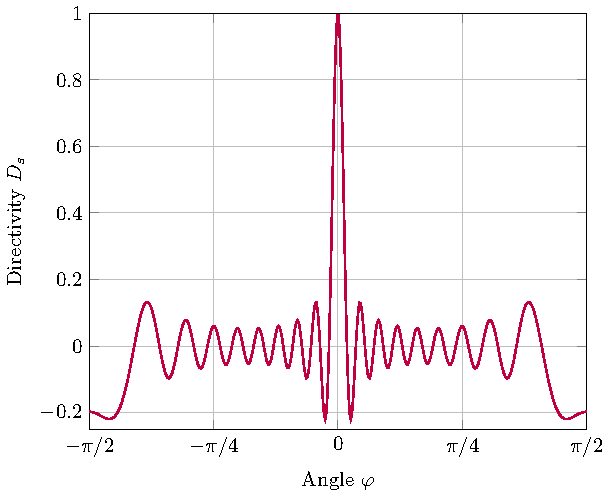
\includegraphics[width=\textwidth]{images/3_Parametric_array/Directivity_NoSteer_Lambda.pdf}
    \caption{Array Directivity $s = \lambda$}
    \label{3_subfig:directivity_no_steer_lambda1}
    \end{minipage}
    \begin{minipage}{0.49\textwidth}
    \centering
    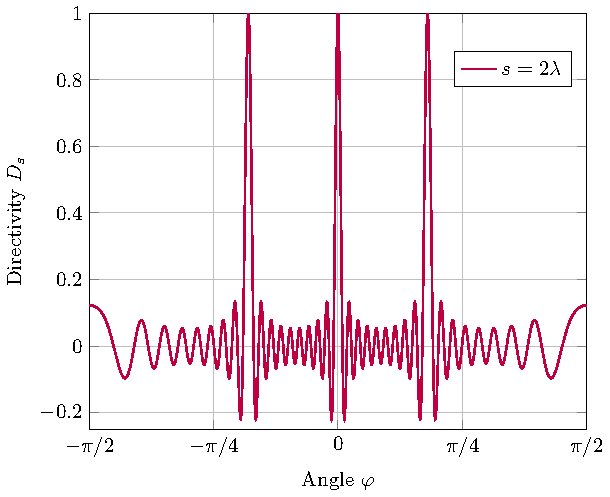
\includegraphics[width=\textwidth]{images/3_Parametric_array/Directivity_NoSteer_2Lambda.pdf}
    \caption{Array Directivity $s = 2\lambda$}
     \label{3_subfig:directivity_no_steer_2lambda}
    \end{minipage}
\end{figure}

\subsection{Beam Steering}
The basic idea of beam steering is to delay the different channels in such a way that the wave fronts create a certain angle. This can be seen graphically in Figure \ref{3_fig:basic_idea_beamforming}.
If the delays are
\begin{equation}
    \Delta t_m = \frac{s \sin{\theta}}{c} \left ( \frac{2m - 1 - M}{2}\right ),
\end{equation}
where $\theta$ is the angle to steer and the weights $C_m = 1$ are inserted into Equation \ref{3_eq:beam_model_final}.
The array directivity $D_S$ turns out to be \cite{alma99116706330905515}
\begin{equation}
    D_S(1, \bm{\Delta t} , \varphi) 
    = 
    \frac{\sin{\frac{Mks(\sin{(\phi)} - \sin{(\theta)})}{2}}}{M\sin{\frac{ks(\sin{(\varphi)} - \sin{(\theta)})}{2}}}.
\end{equation}
This shows that the beam Steering just moves the the directivity calculated in \ref{3_eq:directivity_no_delay} around.  
This can be seen in Figure \ref{3_fig:directivity_beamsteering} for different steering angles.  
\begin{figure}
    \begin{minipage}{0.49\textwidth}
        \centering
        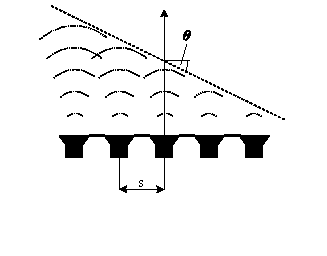
\includegraphics[trim=0mm 7mm 0mm 0mm,width=\textwidth]{images/3_Parametric_array/Beamforming.pdf}
        \caption{Basic Idea of Beam Forming}
        \label{3_fig:basic_idea_beamforming}
    \end{minipage}
    \begin{minipage}{0.49\textwidth}
        \centering
        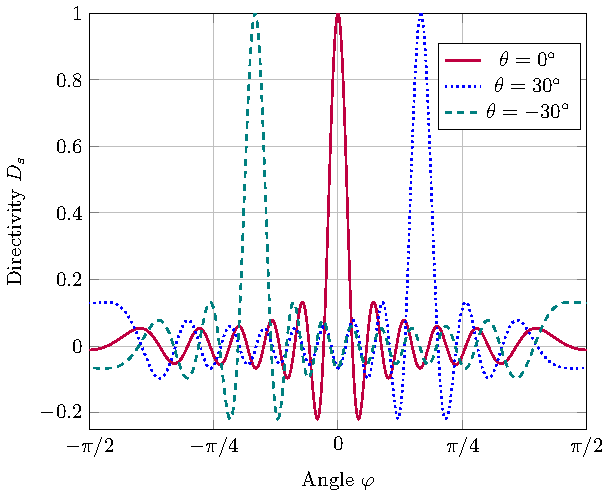
\includegraphics[width=\textwidth]{images/3_Parametric_array/Directivity_Steer.pdf}
        \caption{Array Directivity with Beam Steering}
         \label{3_fig:directivity_beamsteering}
    \end{minipage}
\end{figure}
\newpage

\subsection{Beam Focusing}
To focus the beam at a certain distance $R_0$ the delays have to be chosen as
\begin{equation}
    \Delta t_m = \frac{s^2}{2R_0c}(m-1)(M-m).
\end{equation}
This generates delays which are valued in a parabolic shape. This ensures that the waves meet exactly at the focal point, as shown in Figure \ref{3_fig:beamfocusing}.
\begin{figure}[h!]
    \centering
    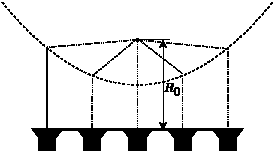
\includegraphics[width=0.55\textwidth]{images/3_Parametric_array/Beamfocusing.pdf}
    \caption{Basic Idea of Beam Focusing}
    \label{3_fig:beamfocusing}
\end{figure}

\subsection{Array Amplitude Weighting}
As explained in Section \ref{2_Acoustics_sec:diffraction_fourier} the diffraction process of a grid can be calculated via the Fourier transform. If an array of transducers is used, the function $s(x)$ is a rectangular sequence. If this rectangular sequence is now sampled with a sampling width of $d$ then the signal becomes a rectangular window known from \acrfull{fir} filters. The main difference being that the time axis is replaced by a spatial axis.

If now weights are applied to the different channels, the rectangular window can be changed to other known window functions, such as Hamming or Hann. The same theories will hold for the main lobe and sidelobes. However, the most commonly used window in array signal processing is the Dolph-Chebyshev window.  
\subsubsection{Dolph-Chebyshev Window}
The Dolph-Chebyshev window is a special window which minimizes the so called Chebyshev norm of the sidelobes for a given main lobe width. The Chebyshev norm is the maximum absolute value
\begin{equation}
    \min_{\omega, \sum \omega = 1} \left \{ \max \left[ | \text{Side lobes}(W(\omega))\right | ]\right \}.
\end{equation}
The transform of the window can be written as
\begin{equation}
    W(\omega_k) = \frac{\cos{ \left [ M \cos^{-1}{\left ( \beta \cos{ \left (\frac{\pi k}{M} \right )} \right)}\right ]}}{\cosh{\left [ M \cosh^{-1}{\left ( \beta \right ) }\right ]}} \qquad k = 0,1,2, \dots, M-1
\end{equation}
Where $M$ is the number of taps of the window and $\beta$ can be used to control the sidelobe level.
If the \acrfull{idft} of $W(\omega_k)$ is taken, the Dolph-Chebyshev window $w(n)$ results.
The controlling of the side lobe level is often done by introducing another variable $\alpha$ which is connected to $\beta$ in the following way
\begin{equation}
    \beta = \cosh{\left [ \frac{1}{M} \cosh^{-1}{\left ( 10^{\alpha} \right ) } \right ]}.
\end{equation}
The maximum side lobe level is now given as
\begin{equation}
    \text{Side lobe level} = L_s =  -20\alpha [dB].
\end{equation}
Whereas the main lobe width is given as
\begin{equation}
    \omega_c = 2 \cos^{-1}{ \left ( \frac{1}{x_0} \right )} \qquad x_0 = \cosh{ \left [ \frac{\cosh^{-1}{\left ( 10^{\alpha} \right )}}{M-1}\right ]}.
\end{equation}
It can be seen that the higher $\alpha$ is chosen, the lower the maximum of the side lobes get. However, the main lobe gets wider.
\begin{figure}[h!]
    \begin{minipage}{0.49\textwidth}
    \centering
    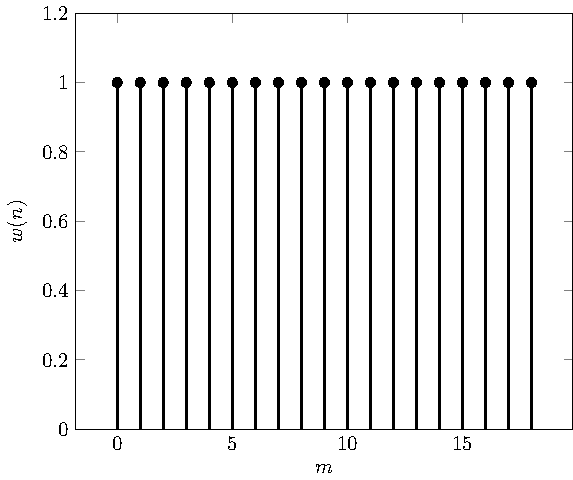
\includegraphics[height=5.3cm]{images/3_Parametric_array/Rectangular_Window.pdf}
    \caption{Channel Weights: Rectangular}
    \label{3_subfig:directivity_no_steer_lambda2}
    \end{minipage}
    \begin{minipage}{0.49\textwidth}
    \centering
    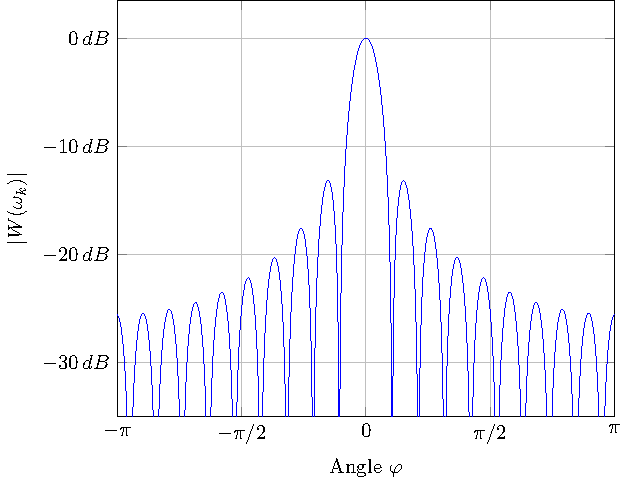
\includegraphics[height=5.3cm]{images/3_Parametric_array/Rectangle.pdf}
    \caption{Directivity Pattern: Rectangular}
     \label{3_subfig:directivity_no_steer_lambda3}
    \end{minipage}
\end{figure}

\begin{figure}[h!]
    \begin{minipage}{0.49\textwidth}
    \centering
    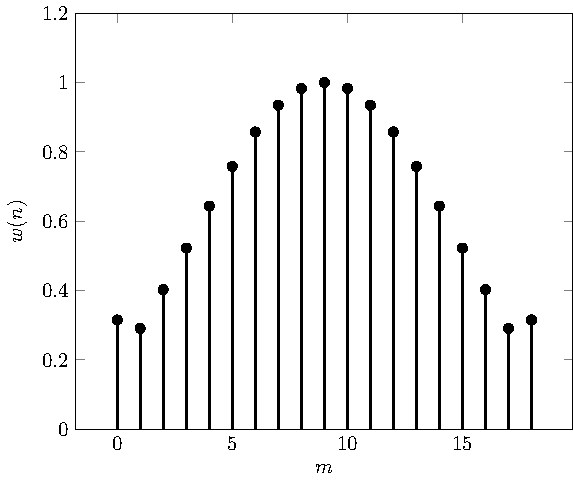
\includegraphics[height=5.3cm]{images/3_Parametric_array/Dolph_Cheby_Window.pdf}
    \caption{Channel Weights: Dolph-Chebyshev}
    \label{3_subfig:directivity_no_steer_lambda4}
    \end{minipage}
    \begin{minipage}{0.49\textwidth}
    \centering
    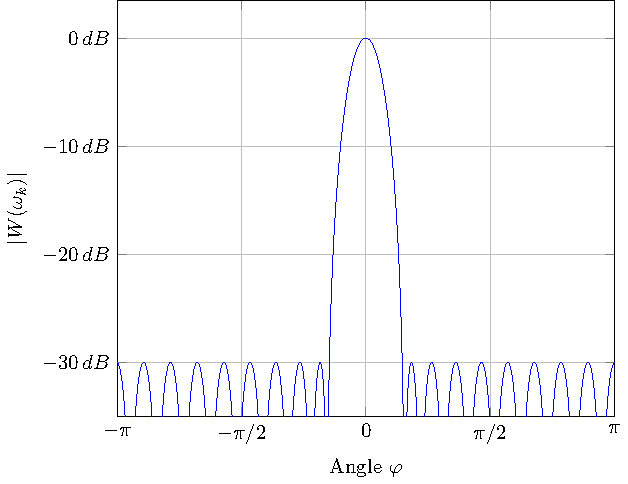
\includegraphics[height=5.3cm]{images/3_Parametric_array/Cheby.pdf}
    \caption{Directivity Pattern: Dolph-Chebyshev}
     \label{3_subfig:directivity_no_steer_2lambda5}
    \end{minipage}
\end{figure}
\newpage





